\documentclass{ximera}
\input{../preamble}
\addPrintStyle{..}
\begin{document}
\author{Alexander Holvoet}
\xmtitle{Basis(sen) definiëren}{}

% Oefeningen: Coördinatentransformaties in ℝ²
% Gebaseerd op coordinate systems visualisatie

\subsection*{Inleiding}
Beschouw de volgende twee coördinatenstelsels in $\mathbb{R}^2$: het zwarte coördinatenstelsel en het blauwe coördinatenstelsel.
In de figuur zijn zes punten aangeduid: $a$, $b$, $c$, $d$, $e$ en $f$.

\begin{figure}[H]
\centering
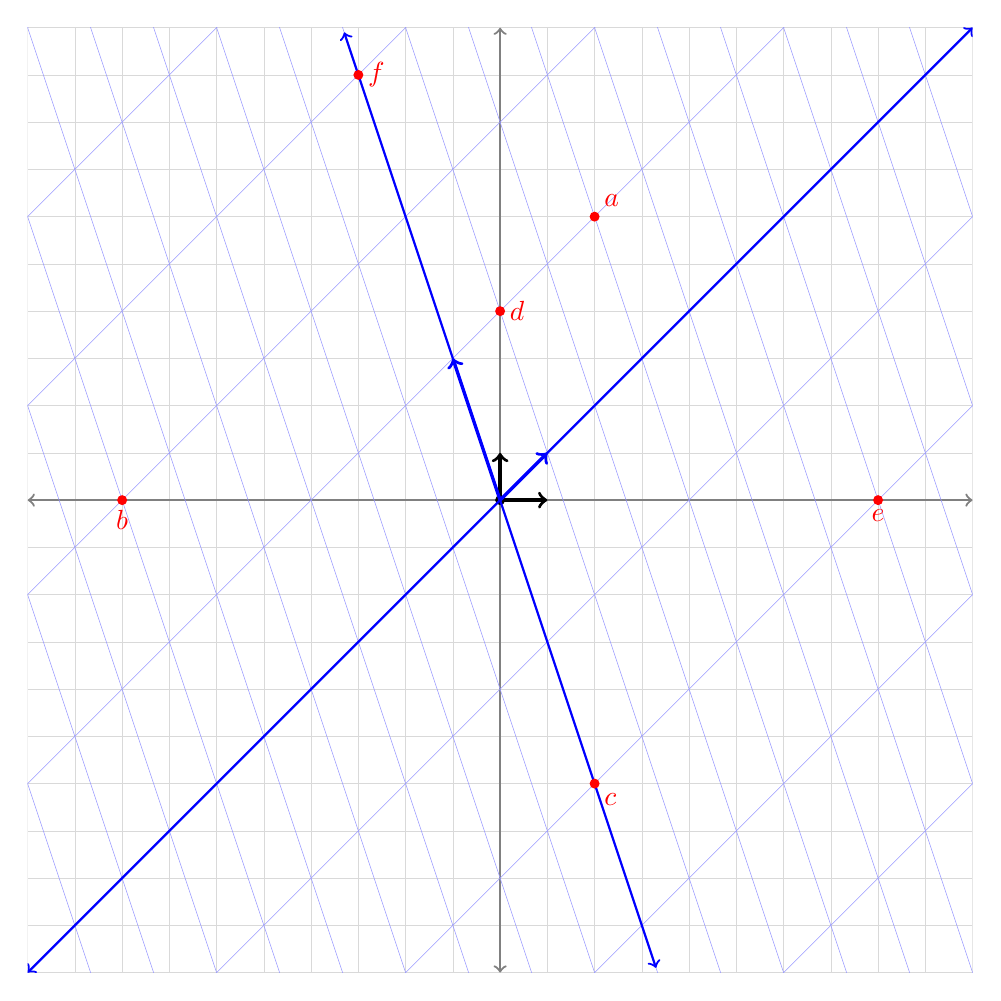
\begin{tikzpicture}[scale=0.6]
    % CLIP EVERYTHING
    \clip(-10,-10)rectangle(10,10);

    % STANDARD COORD SYSTEM
    \draw[gray!30, very thin, step=1] (-10,-10) grid (10,10);
    \draw[gray, thick, <->] (-10,0) -- (10,0);
    \draw[gray, thick, <->] (0,-10) -- (0,10);
    \draw[black, very thick, ->] (0,0) -- (1,0);
    \draw[black, very thick, ->] (0,0) -- (0,1);
    \fill[black] (0,0) circle (3pt);

    % DIFFERENT COORD SYSTEM
    \foreach \k in {-20,...,20} {
    \coordinate (start) at (-10-\k,-10+\k*3);
    \coordinate (end) at (10-\k,10+\k*3);
    \draw[blue!40, very thin] (start) -- (end);
    }
    \foreach \k in {-20,...,20} {
    \coordinate (start) at (-10+\k*1,30+\k*1);
    \coordinate (end) at (10+\k*1,-30+\k*1);
    \draw[blue!40, very thin] (start) -- (end);
    }
    \draw[blue, thick, <->] (-10,-10) -- (10,10);
    \draw[blue, thick, <->] (3.3*1,-3.3*3) -- (-3.3*1,3.3*3);
    \draw[blue, very thick, ->] (0,0) -- (1,1);
    \draw[blue, very thick, ->] (0,0) -- (-1,3);
    
    % RED POINTS
    \fill[red] (2,6) circle (3pt) node[red,above right] {$a$};
    \fill[red] (-8,0) circle (3pt) node[red,below] {$b$};
    \fill[red] (2,-6) circle (3pt) node[red,below right] {$c$};
    \fill[red] (0,4) circle (3pt) node[red,right] {$d$};
    \fill[red] (8,0) circle (3pt) node[red,below] {$e$};
    \fill[red] (-3,9) circle (3pt) node[red, right] {$f$};
    
\end{tikzpicture}
\end{figure}

\subsection*{Vragen}

\begin{exercise}
Schrijf de coördinaten van elk van de bovenstaande punten relatief ten opzichte van zowel het blauwe als het zwarte coördinatenstelsel.
\end{exercise}

\begin{exercise}
Bepaal een matrix die:
\begin{enumerate}
\item coördinaten ten opzichte van het blauwe coördinatenstelsel omzet naar coördinaten in het zwarte coördinatenstelsel.
\item coördinaten ten opzichte van het zwarte coördinatenstelsel omzet naar coördinaten in het blauwe coördinatenstelsel.
\end{enumerate}
\begin{hint}
Als je een coördinaat \(\color{blue}\begin{pmatrix} 2 & 1\end{pmatrix}\) in het blauwe coördinatenstelsel gekregen hebt, dan betekent dat in het zwarte coördinatenstelsel:
\[
2\cdot \begin{pmatrix} 1 \\ 1 \end{pmatrix} + 1 \cdot \begin{pmatrix} -1 \\ 3 \end{pmatrix} = \begin{pmatrix} 1 \\ 5 \end{pmatrix}
\]
\end{hint}
\begin{hint}
De uitdrukking \(2\cdot \begin{pmatrix} 1 \\ 1 \end{pmatrix} + 1 \cdot \begin{pmatrix} -1 \\ 3 \end{pmatrix}\) kan je ook schrijven als:
\[\begin{bmatrix} 1 & -1 \\ 1 & 3 \end{bmatrix} \cdot \begin{pmatrix} 2 \\ 1 \end{pmatrix}\]
\end{hint}
\begin{oplossing}
Om van blauw naar zwart om te zetten, vermenigvuldig je de coördinaten met de matrix \(\begin{bmatrix} 1 & -1 \\ 1 & 3 \end{bmatrix}\).\newline
Om van zwart naar blauw om te zetten, vermenigvuldig je de coördinaten met de inverse van die matrix, namelijk \(\begin{bmatrix} \frac{3}{4} & \frac{1}{4} \\ -\frac{1}{4} & \frac{1}{4} \end{bmatrix}\).
\end{oplossing}
\end{exercise}

\end{document}